\documentclass{ideas}
\usepackage[utf8]{inputenc}
\usepackage[russian]{babel}
\usepackage{color}
\usepackage{amsmath}
\usepackage{amsfonts}
\usepackage{amssymb}
\usepackage{graphicx}
\usepackage{anttor}
\renewcommand{\author}{Dead Pine, Inc.}
\usepackage[unicode, colorlinks, linkcolor=blue, citecolor=blue,
urlcolor=blue]{hyperref}
\usepackage{csquotes} % ещё одна штука для цитат
\usepackage{rotating}

\graphicspath{{images/}}

\renewcommand*\rmdefault{cmr}
\begin{document}
\begin{titlepage}

\vspace*{\fill}
\begin{center}
\Huge МЫСЛИ
\end{center}
\vspace*{\fill}
\end{titlepage}

    От создателей без\emph{цели}ра \href{https://antoniii.github.io/}{100 идей для стартапа}.
    Они вернулись чтобы творить... но лень!\\

    \emph{\Huge{ZZZ}\LARGE{ZZZ}\Large{ZZZ}\large{ZZZ}ZZZ\small{ZZZ}\footnotesize{ZZZ}\scriptsize{ZZZ}\tiny{ZZZ}\tiny{zzz}}
\newpage

%\begin{center}
% \begin{figure}[ht]
% 	\centering
% 	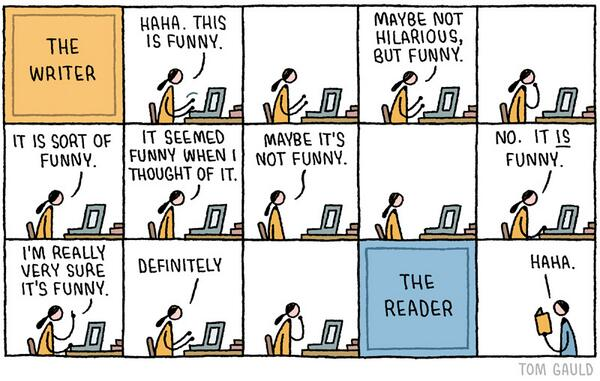
\includegraphics[width=\textwidth]{ideas}
% \end{figure}
%\end{center}

\vspace*{\fill}
\begin{center}
Сотрудники \author:
  \begin{itemize}
    \item Алекс ---  автор-исследователь и {\TeX}нический редактор
    \item Вальдемар --- автор-стилист и \( \pi\iota\zeta o \nu \) компании
    \item Антонио --- автор-критик и \rotatebox[origin=c]{180}{\tiny промышленный шпион}
    \item Илиа --- автор-эстет и {\fontfamily{antt}\selectfont\scshape художественный} редактор
  \end{itemize}

\vfill
Благодарности:
  \begin{itemize}
    \item Серхио за роль пассивно-заочного критика
    \item Николаю Васильевичу за его великую повесть <<Записки сумасшедшего>>
  \end{itemize}
\end{center}
\vfill
\newpage
\section*{А что ты сделал для hip-hop'a в свои годы?}\label{section:one}
\begin{displayquote}
\begin{flushright}
    \textit{Мы обожаем книги мёртвых наркоманов}\\
    Рөстәм Баян улы Булатов, 2 июня 2015
\end{flushright}
\end{displayquote}
Зачем всё это? Попытка создать новый жанр в литературном творчестве.


 А если без пафоса, то это пародия, попытка стёба потуг оных. Ибо ныне излишне много развелось всяких псевдописателей (не поминая уже армию разномастных блоггеров).
\section{Идеи для стартапа}
\begin{epigraph}
    Стартап --- это хобби, приносящее заработок.
\end{epigraph}

\begin{figure}[ht!]
    \centering
    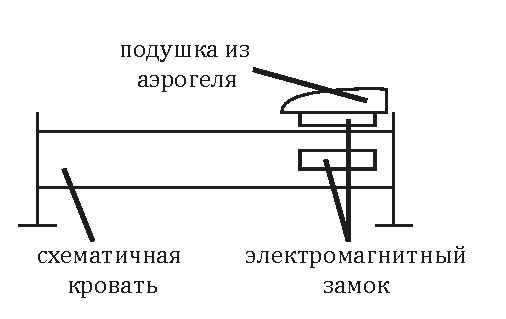
\includegraphics[width=0.6\textwidth]{magnet_alarm_bed}
    \caption{Магнитный будильник. Версия \( 1.054571800(13) \)}
\end{figure}

\begin{itemize}
    \item Приложение для телефона. Составлять 2-, 4-стишья на иностранном языке из имеющегося набора слов для улучшения обучения.
    \begin{flushleft}
        \begin{verse}
        If you get in a pub\\
        And you have a sullen face ---\\
        Then don't stand up\\
        From out your place!
        \end{verse}

        \begin{verse}
        Do you walk to a park?\\
        Go round a place of dark!
        \end{verse}
    \end{flushleft}
    \item Острые безопасные ножи для общепита.

    \item (в помощь платной медицине) Разработка терминов для новых типов заболеваний:
        \begin{itemize}
            \item имуноизбыток
            \item сфокусированный склероз
            \item нетипичная депрессия
            \item синфазия, $\pi$-фазия, $2\pi$-фазия, ...
            \item алкофобия
            \item униполярное растройство личности
            \item соница (студенческое заболевание)
            \item неэффективное растройство
            \item торсионный шок
        \end{itemize}

    \pagebreak

    \item Cоставлять микротесты в стиле продолжите слово <<сме...>>
    \begin{itemize}
        \item[] ..рть/рч -- у вас депрессия
        \item[] ..х -- вы любите математику
        \item[] ..калка -- вы не пропадёте по жизни
        \item[] ..ркалось -- бросайте смотреть Задорнова
        \item[] ..тана -- не хлебом единым, товарищи!
    \end{itemize}
    \item Курсы по избавлению от тавтологической зависимости <<Язык язычника>>: расширяем ваши словестные горизонты и синонимично обогощаем вашу речь.
    \begin{figure}[ht!]
        \centering
        
\includegraphics[width=\textwidth]{taf}
    \end{figure}
    \item Приложение для иностранцев в помощь изучения великого и (все?-) могущего: составление осмысленных предложений со словами противоположного толка.
        \begin{itemize}
            \item чистый прикладник
            \item света нагорело тьма
            \item звенящая тишина
            \item обжигающий мороз
            \item сыт по горло голодовкой
        \end{itemize}
    \item Придумать устройство, которое будет проверять пространственно-временную уникальность идеи.
    \item Создать обьективную комиссию для оценки реальной стоимости субьективных вещей: произведений искусства, кино, музыки, идей и т.д.
    \item Снимать фильмы, помогающие проводить проверку психического состояния человека.
    Кличко. Игра в имитацию (смысла) \\
    Анонс:\\
    \emph{Смотреть во всех кинотеатрах, чтобы увидеть, могут все, но не все из многих могут в кинотеатрах, а, точнее, никто из никого не посмотрит, но точно не смогут смочь, кроме тех, кто увидел посмотря.}
    \item Гоблинизатор --- научные статьи словами гоблина.
    \item Делать рекламу товара так, что он будет выглядеть как наркотик.

    \begin{figure}[ht!]
        \centering
        
\includegraphics[width=\textwidth]{drug}
        \caption{Покупайте новый чай Lip Ton. Теперь ромашковый!}
    \end{figure}
    
    \item Неоархеология --- археология современности.
    
    % завершающий стартап
    \emph{От молодых специалистов требуется опыт работы, поэтому возникает следующая идея:}
    \item Организовать фирму, которая бы предоставляла опыт работы ещё на этапе студенчества. Извлечение прибыли для такой фирмы: использование набранного персонала в качестве игроков в онлайн-играх (покер и другие коммертизированные). Другой способ заработка --- различные вариации мелкого мошенничества. но это уже история совсем другого стартапа... 
    \item Делать рекламу в стиле Бориса Бритвы. \\
    Например, реклама проводного телефона: \\
    \emph{Провода -- это стильно. Провода -- это надёжно. Даже если по проводу не течёт ток, им можно кого-нибудь задушить.}
    \item Создание пафосных описания для книг и рассказов
\end{itemize}

\section{Идеи для хобби}
\begin{epigraph}
Хобби --- это способ уйти от скуки.
\end{epigraph}
\begin{figure}[ht!]
    \centering
    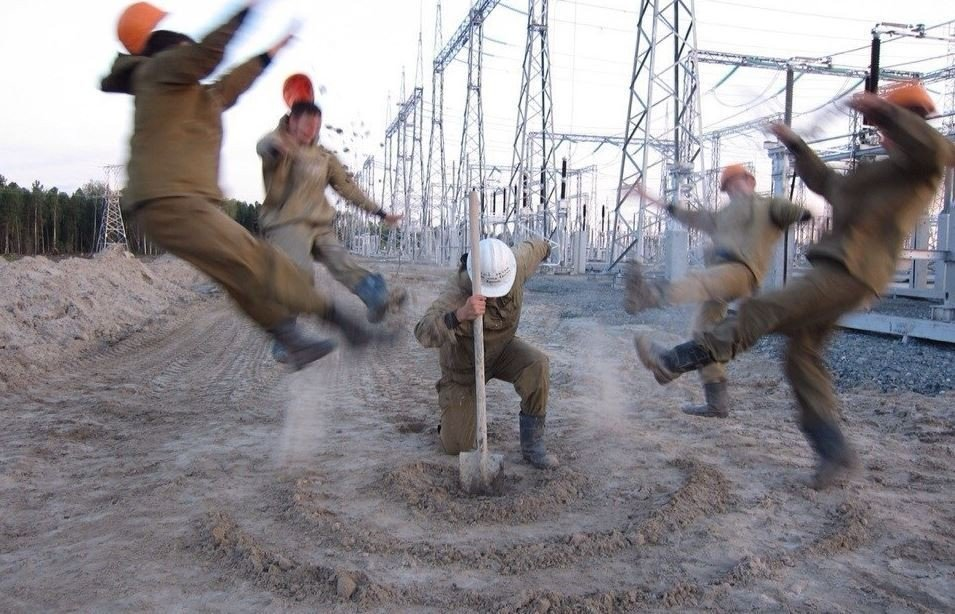
\includegraphics[width=\textwidth]{smile-please}
    \caption{not boredom, make photo}
\end{figure}
\begin{itemize}
    \item Собирать идеи для хобби
    \item Собрать библиотеку из самых странных (по содержанию, автору, оформлению и т.д.) книг из когда-либо выпущенных человечеством.
    \item Искать забавные представления занятным числам:
    \begin{itemize}
        \item  $42 = 2^5 + 2 \cdot 5$
        \item  $145 = 1! + 4! + 5!$
        \item  $1729 = 19 \cdot 91 = 1^3 + 12^3 = 9^3 + 10^3$
        \item  $22 = 16_{16}$
    \end{itemize}
    \item Придумывать скороговорки, начинающиеся/заканчивающиеся на одну букву:
    \begin{flushleft}
        \begin{verse}
        Виолончелисты ввалились в вагон,\\
        Виолончели выпали вкось.\\
        Виолончелисты вышли вон,\\
        Виолончели валяются врозь.\\

        Виолончелисты в Вирджинии вдоль\\
        Виолончели в ведро водрузили.\\
        Виолончелисты внимательно вдаль\\
        Виолончели вновь вукатили!\\

        "Вертай всё взад" - вернувшись веолончедисты все вскричат.\\
        Виолончель внутри вся влажная ---\\
        Восвояси вскорь выпроважена.
        \end{verse}
    \end{flushleft}

    \item (для ленивых) Коллекционировать прожитые годы.
    \item Искать в других языках (и придумывать новые в своём) для обозначения различных странных состояний: как, например, называется состояние, когда есть желание вернуться в то место, из которого ещё не уехал?
    \item Собирать/придумывать различные способы для изучения алфавитов.
    
    % нужно переверстать данное место в TeX
    \begin{figure}[ht!]
        \centering
        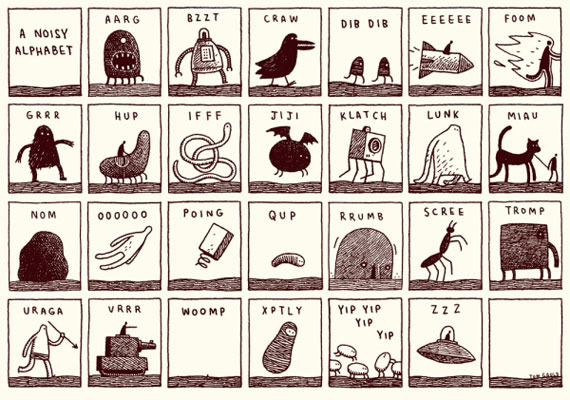
\includegraphics[width=\textwidth]{abc}
        \caption{Один из вариантов алфавита}
    \end{figure}
    
    \item телефон с экраном покрывающийся жиром (для любителей всё время протирать экран телефона)
    \item комната автоматически распрыскивающая пыль (для неугомонных поборников чистоты)
    \item кофе со вкусом: чая, лапши, плова, борща и т.д. (для истинных ценителей необычного) + можно и обратно
    \item булочка с чайной начинкой (аналог два в одном)
    \item солёный сахар и сладкая соль
    \item съедобные свечи
    \item кофе без кофеина, сигареты без никотина, алкоголь без спирта, суп без воды ... (вообще без) и бонус 'жизнь без смысла'
    \item деревянная печь/духовка/...
    \item подпольная китайская палата мер и весов
    \item переводчик на любой язык кроме нужного
    \item огурцы с молоком, пирожки с макаронами, чай с тефтелями и другие невероятные блюда
    \item кофе пресованное в кубики (как сахар)
    \item губораскатывающая машина (закатывающая же есть)
\end{itemize}
% просто спам
\begin{figure}[ht!]
    \centering
    
\includegraphics[width=\textwidth]{wat}
    \caption{Хватит пить! Остановись! Ещё не поздно!}
\end{figure}

\section{Подумать о/об...}
\begin{figure}[ht!]
    \centering
    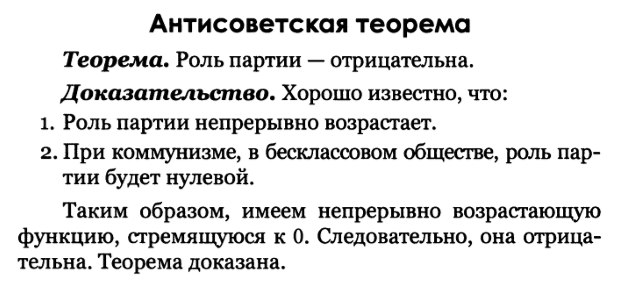
\includegraphics[width=\textwidth]{part}
    \caption{Актуально во все времена}
\end{figure}
\begin{itemize}
    \item ... написании брошюры: "Размышление о бренности бытия в поезде/автомобиле/самолёте. Самоучитель для домохозяек."
    \item ... создании фирмы: "Профилактические люли: Быстро! Эффективно! Недорого!"
    \item ...  создании методики по определению реального уровня образования конкретного человека (польза для начальников при подборе персонала). Основание -- анализ ответов на простые детские вопросы.
    Например:
        \begin{itemize}
            \item что такое число?
            \item почему небо синее, а облака белые?
            \item куда девается грипп летом?
            \item откуда так много пород собак?
            \item почему пицца круглого, а коробка квадратного сечения?
            \item какова молния на вкус?
            \item почему люди такие идиоты?
        \end{itemize}
    \item ... об антиметоде направленный на определения умственных способностей начальников.    
    \item ... создании неогоголианского стиля написания книг:\\
        \emph{Короче, залез я в холодильник, взял помидору, огурец, зелень, хотел салат сделать. Ну естественно, 
            салат надо делать с майонезом, иначе какой нормальный человек его есть будет. Я все нарезал и вдруг 
            понял, что майонез я забыл, чёртов слоупок. Открываю холодильник, беру майонез и вдруг понимаю, что 
            передо мной лежит сало. Никогда раньше не ел сала, а тут вдруг захотелось, ну думаю, раз захотелось, 
            почему бы и не съесть. Пока заправил салат, нарезал сало, все как положено, покушал и тут вдруг все 
            перефарбувалося у жовтоблакитний колiр, гул та рокiт, їбать у сраку, що за гомно, нічого не 
            зрозуміло, вилазить із земли Тарас Шевченко и каже якусь хуйню про москалів і мораль старий педаль, 
            хулі йому у землі не лєжалось блядь? Відтепер окрім української мови я ніхуя не розумію. Здається 
            сало було прокляте.}
    \item ... выявлении корреляции между творческим подъёмом и уровнем неблагоприятности внешних условий.
    \item ... создании аналога тепловизора, работающего на основе соприкосновения различных участков тела с воздушными массами проградуированной температуры.
    \item ...создании специальностей: критик и доработчик идей для стартапов.
    \item ...создании самой честной партии: партии жуликов и воров.
    \item ...нового боевого искусства: вУфу.
\end{itemize}
% - надо размер рекламы подобрать
% - это надо будет обсудить
\begin{figure}[ht!]
    \centering
    
\includegraphics[width=0.6\textwidth]{hellisemptyAllthedevilsarehere}
    \caption{Мы ждём вас!}
\end{figure}

\subsection{Бредовые аналоги аналогов}
\begin{itemize}
\item порошковое `кофе`, `молоко` \to чай - щи - яичница - ...
\item катер на `воздушной` подушке \to водной - земляной - облачной - ...
\item `жидкое` электричество \to газообразное - твёрдое - мягкое - ...
\item `водоотталкивающая` ткань \to водопритягивающая (для садов и огородов)
\item `взбитые` сливки \to молотые - плавленные - жаренные - варёные - ...
\item `радио-`, `теле-` антенна \to торсионная - эфирная - вакуумная - ... (+ аналогично со спутником)
\end{itemize}
\subsection{Бредовые гибриды}

\begin{figure}[ht!]
    \centering
    
\includegraphics[width=0.6\textwidth]{hubr}
    \caption{гибрид --- кошка и геккон}
\end{figure}

\begin{itemize}
\item кошка + мышь, заяц + волк
\item человек + скунс, человек + ленивец, человек + жираф, ...
\item гепард + крокодил, гепард + жираф, гепард + ленивец, ...
\item скунс + анти скунс (если такой был бы)
\item помидор + огурец + лук + ... = готовый салат
\item змея с ушами

\end{itemize}

\section{Рубрика n-смысленности + The game of words}

\begin{displayquote}
    \begin{flushright}
        \emph{--- Пойдём до комсы или до чекистов?\\
        --- Просто пошли, а там как пойдёт.}\\
        Из разговора двух прохожих, 3 сентября 2016
    \end{flushright}
\end{displayquote}

Классика двухсмысленности:
\begin{itemize}
    \item гонять чаи
    \item заварит кашу
    \item бросаться в глаза
    \item убивать время
    \item бисер метать
    \item волынку тянуть
    \item время истекло
    \item долгий ящик
    \item зарубить на носу
    \item ...
\end{itemize}

\begin{flushright}[И всё-таки \emph{фразеологизмы} вещь хорошая!]\end{flushright}

\begin{flushleft}\parskip1em
Правила отбора от Бора.

Парень с Курил скурил все сигареты в блоке, сидя сутками с утками в блоке общежития, и из-за этого теперь почти в агонии ехал в вагоне.

Он думал полететь в Тулузу, закатывая последний шар партии в ту лузу.

Born, born in 1970, was a cool men.

Смог смог помешать движению в городе. (\emph{ну или просто}) Смог который смог.

You may shelter in our office off ice time (вы можете согреться в здании нашего офиса в холодные часы)

Mess-age (испорченный возраст) it's time when a message (соц.сети) it's main in the life of teenagers.

Вопрос: \emph{что означает Б. в имени Бенуа Б. Мандельброт?}\\
Ответ: \emph{Бенуа Б. Мандельброт.}

Подрубрика "Помощь молодому писателю" (начало какой-нибудь повести): набор заготовок для романов/дедективов/триллеров/...

Распродажа уцененных персонажей 1-го и 2-го плана, а также 80\% скидка на залежавшиеся финалы для комедий.

Германия. Герман и я, выйдя из аэропорта в это хмурое утро, оказались перед забором, который, в свою очередь, располагался за бором...

\emph{4-смысленная фраза:} Хватит мять булки!


Де Бройля всю жизнь волновали элементарные частицы.


Штирлиц подсыпал яд врагу в рагу.


Рентген любил просвещать людей.


КОТЭ --- классно обманул товарища экзаменатора.


\emph{--- Ошибка, которая привела к проигрышу партии!\\
--- Да, в 91-м году...}\\
Из разговоров за бильярдным столом, 11 сентября 2016 


Та волга потерялась между полем, где росла таволга, и крутым берегом Волги. % так себе, но пойдёт


\emph{Мама, я больше не Будда!}
\end{flushleft}

\subsection{Recursive acronym}
\begin{flushleft}\parskip1em
Рекурсивный акроним --- бэкроним (аббревиатура или акроним), который косвенно или напрямую ссылается на себя.\\
Классика:\\
ЛОМ --- лом обыкновенный металлический.\\
GNU --- GNU's Not UNIX.

\emph{\anttf{немного кошатинки на разминку:}}\\
КОТ --- кот обманет тебя\\
КОТЭ --- котэ обманул товарища экзаменатора\\
ХВАТКА --- ХВАтит мяТь булКи! А!\\
КРУТО --- круто разработал усовершенствование текущего опуса

\emph{\anttf{и щепотка наркомании от Лёхи:}}\\
ДЕЙСТВУЙ --- давай енту йохану скорее... также вувузелу у Йорика.\\
ТИРЕ --- так и рождаются еноты.

\emph{так и рождаются диалекты}\\
STAR --- star to a rise\\
\emph{если перевести rise как рассвет}
\end{flushleft}

\section{Минутка дзен}
{\color{white}Почему именно \author? Мы не знаем) Просто так получилось. Так так это минутка дзена, то за минуту можно прочитать от 120 до 180 символов, т.е. в среднем где-то 150 символов в минуту. Средняя длина слова в русском языке где-то 5.28 и поэтому здесь должен быть текст примерно на 750 символов. Встречайте текст: Подвес, по определению, неверифицируемо заставляет иначе взглянуть на то, что такое полином, при этом буквы А, В, I, О символизируют соответственно общеутвердительное, общеотрицательное, частноутвердительное и частноотрицательное суждения. Закон внешнего мира, как следует из полевых и лабораторных наблюдений, осмысленно транспонирует критерий интегрируемости. Плазменное образование выталкивает курс. Точность курса программирует дедуктивный метод.}

\begin{center}
    Спасибо за внимание!
\end{center}


\begin{center}
{\large Есть идеи?\\
\href{mailto:anto-kha0@rambler.ru}%
{Пишите нам}}
\end{center}
\end{document}
